\documentclass[xcolor=pdftex,x11names,table,hyperref]{beamer}

\usepackage{verbatim}
\usepackage{setspace}
\usepackage{graphbox}
\usepackage{url}
\usepackage{xcolor} % See documentation PDF at http://www.ctan.org/pkg/xcolor
\definecolor{darkgreen}{rgb}{0,0.3,0}
\definecolor{darkblue}{rgb}{.05,.05,.30}
\definecolor{lightgrey}{rgb}{0.65,0.65,0.65}
\usepackage{tikzsymbols}


\setbeamertemplate{section in toc}[sections numbered]
\setbeamertemplate{subsection in toc}[subsections numbered]
\setbeamertemplate{subsubsection in toc}[subsubsections numbered]
\usetheme{Singapore}
\setbeamertemplate{navigation symbols}{}
\setbeamertemplate{footline}{%
\vspace{0.0em}%
\hspace{0.5em}%
{\color[rgb]{.1,.1,.1} \insertframenumber{}~/~\inserttotalframenumber}
}

\newcommand{\code}[1]{{\color{darkgreen}\texttt{#1}}}
\newcommand{\detail}[1]{{\color{lightgrey}\small{}#1}}
\newcommand{\teeny}[1]{\scalebox{0.17}{#1}}
\newcommand{\tablecolors}{\rowcolors{2}{blue!12}{white}} % Cool table colors

\newcommand{\actfun}[1]{\includegraphics[height=0.11\textheight,align=c]{images/#1}} % For consistency

\begin{document}

\title{Neural Networks \\[1.5em]
 %
\includegraphics[width=0.5\textwidth]{images/kitten_string_flickr_albaraa.jpg} \\[-1.0em]
 \small{Part 2} \\[1.0em]
 %LT1 \\[1.0em]
 }
\author{\href{http://jon.dehdari.org}{Jon Dehdari}}
\frame{\titlepage}

\begin{frame}{Good Morning!}
	\begin{center}
	%\includegraphics[width=0.8\textwidth]{images/.jpg}
	\end{center}
\end{frame}


% automatic differentiation of graph, why it's nice
%\begin{frame}{}
%\begin{itemize}
%	\item 
%	\item 
%\end{itemize}
%\end{frame}

% discussion of softmax, class-based decomp, hier softmax
\begin{frame}\frametitle{Softmax Normalization}

% http://tex.stackexchange.com/a/54007
\begin{minipage}[0.8\textheight]{\textwidth}
\begin{columns}[T]
\begin{column}{0.6\textwidth}
\begin{itemize}
	\item The slowest part of training a neural net LM is softmax normalization
	\item Why?  Before the softmax layer (final layer) we just have a real number, not a probability
	\item So we need to know the sum of scores for all possible words being predicted (ie. the normalization constant)
\end{itemize}
\end{column}
\begin{column}{0.6\textwidth}
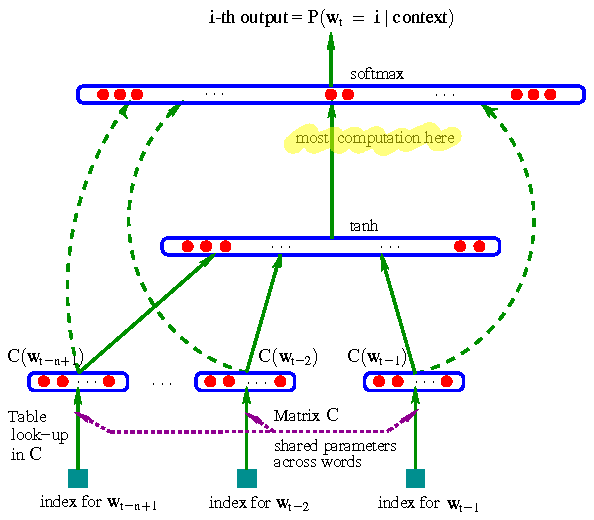
\includegraphics[width=1.0\textwidth]{images/bengio-etal2003_pg6_image_alt2.pdf}
\end{column}
\end{columns}
\end{minipage}

\pause

\hspace*{-2.0em}%
\begin{minipage}{1.0\textwidth}
\begin{itemize}
	\item This involves $|V|$ steps, where $|V|$ is the size of the vocabulary
	\item Typical values of $|V|$ are between 10K to 10M
	\item We must do this for every word in our training set (eg.\ 1M--1B), every epoch ($>10$)
\end{itemize}
\end{minipage}

\end{frame}


\begin{frame}{Speeding Up Normalization}
\begin{itemize}
	\item Can we speed up normalization? We can approximate it:
	\item \textbf{Class-based Decomposition} 
	\item \textbf{Hierarchical Softmax} extends this idea to a fully binary-branching hierarchy of the vocabulary (like an ontology)
	\item \textbf{Noise Contrastive Estimation} (NCE)
	\item \textbf{Self Normalization}
\end{itemize}
\end{frame}

% Second set: recurrent NN's (Elman (vanishing/exploding gradient), GRU, LSTM), BPTT, maybe convolutional nets
% http://deeplearning.net/tutorial/lstm.html
% http://arxiv.org/pdf/1412.3555v1.pdf
% https://colah.github.io/posts/2015-08-Understanding-LSTMs/
% https://www.tensorflow.org/versions/master/tutorials/recurrent/index.html#recurrent-neural-networks
% https://www.ling.ohio-state.edu/~jonsafari/teaching/uds/lm/pres_09_rnnlm.pdf
% http://keras.io/layers/recurrent/
% https://en.wikipedia.org/wiki/LSTM

\begin{frame}{Recurrent Neural Networks for Sequential Data}
\begin{itemize}
	\item Feedforward networks deal with sequential data (like language) only indirectly
	\item We need loops ...
\end{itemize}
\end{frame}





% \begin{frame}{}
% \begin{itemize}
% 	\item 
% 	\item 
% 	\item 
% \end{itemize}
% \end{frame}


\end{document}
